\chapter{Estación de monitoreo de campo eléctrico}
\label{ch:background}

La estación tiene como fin observar, medir, codificar y transmitir las variables atmosféricas que apoyen el estudio de los mecanismos de aceleración de partículas secundarias cargadas. El campo eléctrico atmosférico es la variable más relevante, sin embargo la medición de parámetros como temperatura, humedad y presión permite ampliar el estudio de los fenómenos y eventos relacionados a la generación de campo eléctrico atmosférico, como la altura de la nube, el potencial eléctrico atmosférico y ubicación geográfica de las descargas atmosféricas.

\section{Variables atmosféricas}
Desde la formación de nubes de tormenta hasta la disipación de las misma encontramos algunas variables atmosféricas que nos ayudan a entender los eventos que ocurrieron durante el desarrollo de una tormenta eléctrica e incluso nos permiten predecirlas. La importancia de este proyecto radica en la capacidad de medir el campo eléctrico atmosférico y algunas las variables relacionadas, como la altura de la nube y potencial eléctrico, también resulta de gran relevancia conocer la ubicación de las descargas atmosféricas que producen campos eléctricos transitorios y en general, como se mencionó anteriormente, ayudar al estudio de los mecanismos de aceleración de partículas secundarias cargadas.
\subsection{Temperatura}
El calentamiento de la atmósfera es el resultado del balance entre la radiación entrante y saliente de la superficie terrestre. La mayor parte de la radiación solar incidente es absorbida por la parte superficial del suelo y como consecuencia se torna más caliente que el aire que está en contacto directamente con ella. Por la noche, una cantidad considerable de calor se irradia desde la superficie del suelo y causa un enfriamiento en la parte más superficial del mismo \cite{jaramillo2005clima}.\\

Las corrientes de aire caliente a menudo son provocadas por la misma radiación térmica. Cuando se produce un choque entre un frente frió y una de estas corrientes de aire caliente, se produce una condensación de agua que desemboca con frecuencia en una nube de tormenta, es por esto que se considera relevante para el estudio de la formación de tormentas eléctricas.\\

Para medir la temperatura del aire se utilizó un sensor BME280, voltaje de alimentación entre 1.71 V y 3.6 V, consume 3.6 $\mu$A para un periodo de muestreo de 1 Hz, rango de operación entre -40 $^{\circ}C$ y +85 $^{\circ}C$, posee una resolución de $\pm$0.5 $^{\circ}C$, utiliza I$^{2}$C y SPI como protocolos de transmisión de datos, en la Fig. \ref{bme_t} se muestra el sensor comercial fabricado por la empresa Sparkfun, junto a su tabla de especificaciones tomada del datasheet.

\begin{figure}[h!]
 \centering
  \subfloat[]{
   \label{t1}
    \includegraphics[width=0.25\textwidth]{Figures/bme.jpg}}
  \subfloat[]{
   \label{t2}
    \includegraphics[width=0.75\textwidth]{Figures/bme_tem.PNG}}
 \caption{(a) Sensor BME280 humedad, presión y temperatura. (b) Tabla de especificaciones del sensor, el cual tiene un voltaje de alimentación entre 1.71 V y 3.6 V, consume 3.6 $\mu$A para un periodo de muestreo de 1 Hz, rango de operación entre -40 $^{\circ}C$ y +85 $^{\circ}C$, posee una resolución de $\pm$0.5 $^{\circ}C$, utiliza I$^{2}$C y SPI como protocolos de transmisión de datos.}
 \label{bme_t}
\end{figure}

\subsection{Humedad}
Dentro de la atmósfera el agua puede estar presente como vapor de agua (un gas invisible), como gotas de agua y como cristales de hielo (fases visibles). El vapor de agua ingresa en la atmósfera por evaporación (desde el océano, ríos, lagos), transpiración desde las plantas y sublimación del hielo y la nieve. El vapor de agua es uno de los constituyentes del aire, se caracteriza por ser variable en cantidad, de acuerdo con la disponibilidad de agua y energía y representa hasta un 4$\%$ en volumen del aire. Este volumen es determinado por la temperatura del ambiente, a mayor temperatura del aire hay mayor capacidad de retención de humedad\cite{jaramillo2005clima}.\\

La tormenta es la manifestación extrema de la inestabilidad atmosférica. Se produce con el cumulonimbus y va acompañada de un cierto número de fenómenos tales como descargas atmosféricas  y lluvias. Los requisitos iniciales para la formación del cumulonimbus que desemboca en tormenta, es la presencias de aire húmedo, un gradiente vertical de temperatura y un fuerte mecanismo de elevación para forzar el aire hacia arriba. Cuanto mayores son las diferencias de densidad entre las masas de aire (temperatura y humedad), mayores son las inestabilidades atmosféricas que se desarrollan y mayor es la intensidad de estas tormentas \cite{price2009thunderstorms}.\\

\begin{figure}[H]
 \centering
  \subfloat[]{
   \label{h1}
    \includegraphics[width=0.25\textwidth]{Figures/bme_2.jpg}}
  \subfloat[]{
   \label{h2}
    \includegraphics[width=0.7 \textwidth]{Figures/bme_hum.PNG}}
 \caption{(a) Sensor BME280 humedad, presión y temperatura. (b) Tabla de especificaciones del sensor, su voltaje de alimentación esta entre 1.71 V y 3.6 V, consume 3.6 $\mu$A para un periodo de muestreo de 1 Hz, rango de operación entre 0 $\%$RH y 100 $\%$RH, posee una resolución de $\pm$0.008 $\%$RH, con una tolerancia de $\pm$3 $\%$RH, utiliza I$^{2}$C y SPI como protocolos de transmisión de datos.}
 \label{bme_h}
\end{figure}

Se seleccionó el sensor BME280 para las mediciones de humedad, su voltaje de alimentación esta entre 1.71 V y 3.6 V, consume 3.6 $\mu$A para un periodo de muestreo de 1 Hz, rango de operación entre 0 $\%$RH y 100 $\%$RH, posee una resolución de $\pm$0.008 $\%$RH, con una tolerancia de $\pm$3 $\%$RH, utiliza I$^{2}$C y SPI como protocolos de transmisión de datos, en la Fig. \ref{bme_h} se muestra el sensor comercial fabricado por la empresa Sparkfun, junto a su tabla de especificaciones tomada del datasheet.\\

\subsection{Presión}
La presión atmosférica es la más empleada al estudiar la atmósfera y el aire, se define como el peso que ejerce el aire sobre la unidad de superficie. Se puede obtener una medida de la presión atmosférica en un lugar determinado pero de ella no se pueden sacar muchas conclusiones; sin embargo, la variación de dicha presión a lo largo del tiempo permite obtener una información útil que, unida a otros datos meteorológicos (temperatura atmosférica, humedad y vientos), puede dar una imagen bastante acertada del tiempo atmosférico en dicho lugar e incluso un pronóstico a corto plazo del mismo \cite{blanco1997programa}.\\

Cuando el aire está frío, se contrae, aumenta la densidad y, por lo tanto, desciende, haciendo aumentar la presión y provocando estabilidad barométrica o anticiclónica. Se forma así una zona de calmas, es decir, sin vientos, ya que el aire frío y pesado desciende lentamente en sentido circular y comienza a girar casi imperceptiblemente en sentido horario en el hemisferio norte y antihorario en el hemisferio sur. Se forma, entonces, un anticiclón. Cuando el aire está caliente, asciende, haciendo bajar la presión y provocando inestabilidad. Se forma así un ciclón o borrasca \cite{blanco1997programa}.\\

La presión atmosférica se mide en diferentes unidades. Entre ellas destacamos la atmósfera, el mm de Hg (mercurio) o tor y el milibar. La presión atmosférica normal es de 1.013 mb, pero ésta varía de un día a otro. Se seleccionó el sensor BME280 para las mediciones de presión, su voltaje de alimentación esta entre 1.71 V y 3.6 V, consume 3.6 $\mu$A para un periodo de muestreo de 1 Hz, rango de operación de 30,000 Pa a 110,000 Pa, posee una precisión relativa de 12 Pa y precisión absoluta de 100 Pa, utiliza I$^{2}$C y SPI como protocolos de transmisión de datos, en la Fig. \ref{bme_p} se muestra el sensor comercial fabricado por la empresa Sparkfun, junto a su tabla de especificaciones tomada del datasheet.\\

\begin{figure}[h!]
 \centering
  \subfloat[]{
   \label{p1}
    \includegraphics[width=0.25\textwidth]{Figures/bme_3.jpg}}
  \subfloat[]{
   \label{p2}
    \includegraphics[width=0.75\textwidth]{Figures/bme_press.PNG}}
 \caption{(a) Sensor BME280 humedad, presión y temperatura. (b) Tabla de especificaciones del sensor, su voltaje de alimentación esta entre 1.71 V y 3.6 V, consume 3.6 $\mu$A para un periodo de muestreo de 1 Hz, rango de operación de 30,000 Pa a 110,000 Pa, posee una precisión relativa de 12 Pa y precisión absoluta de 100 Pa, utiliza I$^{2}$C y SPI como protocolos de transmisión de datos.}
 \label{bme_p}
\end{figure}

\subsection{Altura de la nube y potencial eléctrico}
Sabemos que el campo eléctrico lento es producido por la acumulación de carga en las nubes, idealmente el conjunto atmósfera tierra se puede considerar como un capacitor esférico de placas paralelas, por lo que la expresión de la Eq. \ref{potencial} describe el comportamiento del potencial que se genera entre las nubes y la tierra, con $E$ como el campo eléctrico y $d$ la altura de la base de la nube cúmulo.
\begin{equation}
    V = Ed
    \label{potencial}
\end{equation}
G. Lawrence et. al. en su trabajo \textbf{"The Relationship between Relative Humidity and the Dewpoint Temperature in Moist Air"} \cite{lawrence2005relationship}, nos entrega una expresión para la aproximación de el nivel de condensación de elevación LCL, es decir, la altura de la base de la nube cúmulo ($Z_{lcl}$), que está estrechamente relacionado con la temperatura de rocío ($t_{d}$) y la temperatura del aire ($t$) a nivel de suelo tal como se observa en la Eq. \ref{alt}.
\begin{equation}
    Z_{lcl}\approx 125\left (t - t_{d}\right )
    \label{alt}
\end{equation}
La temperatura a la que se condensa (o solidifica) el vapor de agua en una muestra de gas a un valor de presión se le llama temperatura de punto de rocío ($t_{d}$) y su valor depende de la humedad relativa del gas ($RH$) \cite{lawrence2005relationship}, tal como se observa en la Eq. \ref{td}.
\begin{equation}
    td \approx t - \left ( \frac{100 - RH}{5}\right)
    \label{td}
\end{equation}

\section{Sistema de posicionamiento}
La estación de monitoreo, posee un sistema GPS que permite conocer el tiempo y ubicación de los eventos registrados, esto es importante para correlacionar eventos que ocurrieron en la misma franja temporal. El GPS utiliza los datos suministrados por al menos 4 satélites en orbita para conocer el tiempo y calcular su ubicación espacial.\\

El GPS que se utilizó en la estación es el Venus638FLPx de la compañía Sparkfun (ver Tabla. \ref{cara_gps}), por su tamaño, potencial y versatilidad, utiliza protocolo de comunicación serial a 9600 baudios, posee una velocidad de actualización de hasta 20 Hz con precisión de 2.5 m, se alimenta con 3.3 V y posee un pin para conexión de una batería externa o un supercondensador a la placa, para admitir reinicios rápidos después de desconectar la alimentación.\\

\begin{table}[]
\resizebox{\textwidth}{!}{%
\begin{tabular}{|c|c|}
\hline
\cellcolor[HTML]{FFFFC7}\textbf{CARACTERÍSTICAS} & \parbox{2cm}{\includegraphics[width=0.2\textwidth]{Figures/gps_venus.jpg}} \\ \hline
20 Hz de tasa de actualización & -148dBm  de sensibilidad de arranque en frío \\ \hline
Sensibilidad de seguimiento -165dBm & 29 segundos de arranque en frío TTFF \\ \hline
TTFF de 3,5 segundos con AGPS & 1 segundo arranque en caliente \\ \hline
Precisión de 2.5m & Detección y supresión de múltiples rutas \\ \hline
Detección y mitigación de atascos & Soporte SBAS (WAAS / EGNOS) \\ \hline
Efemérides extendidas de 7 días AGPS & Navegación a plena potencia de 67 mW \\ \hline
Funciona directamente con antena activa o pasiva & Flash interno para el registro opcional \\ \hline
Contiene LNA, filtro SAW, TCXO, RTC Xtal, LDO & Sin RoHS compatible con Pb \\ \hline
\end{tabular}%
}
\caption{Características del GPS Venus638FLPx de la compañía Sparkfun.}
\label{cara_gps}
\end{table}
El GPS suministra 6 tramas de datos llamadas NMEA, de las cual se puede obtener el tiempo, fecha, ubicación, cantidad de satélites, altitud entre otros. Las tramas que se analizan para el proyecto son la GGA (Global Positioning System Fix Data) y la RMC (Recommended Minimum Specific GNSS Data). De la trama GGA se obtiene una cadena de datos tal como se muestre en la Fig. \ref{GGA}, de donde se extrae el tiempo UTC (hhmmss.sss), latitud (ddmm.mmmm), indicador N/S (a), longitud (dddmm.mmmm), indicador E/W (a) y altitud (a).\\

\begin{figure}[H]
\begin{center}
\includegraphics[width=.8\textwidth]{Figures/GGA_RMC.png}
\caption[Trama de datos del GPS]{Trama de datos GGA y RMC suministrada por el GPS venus a una frecuencia de 1 Hz. De la trama GGA se obtiene el tiempo UTC (hhmmss.sss), latitud (ddmm.mmmm), indicador N/S (a), longitud (dddmm.mmmm), indicador E/W (a) y altitud (a), de la trama RMC se obtiene la fecha UTC (ddmmyy).}
\label{GGA}
\end{center}
\end{figure}
Existen varios métodos para determinar la ubicación de una descarga atmosférica, entre ellos tenemos técnicas de búsqueda de dirección (DF) \cite{krider1976gated}, tiempo de llegada (TOA) \cite{lee1989ground}, una combinación de estos dos \cite{cummins1998combined} y métodos de interferometría \cite{hayenga1981two}. Para el proyecto se utilizó una variación del método de tiempo de llegada (TOA), llamado algoritmo de trilateración el cual consiste en un método matemático para calcular un punto en el espacio usando distancias desde diferentes puntos de referencia a otras entidades geométricas conocidas, el número mínimo de entidades para poder aplicar el método es de 3, esto es tener una red espacialmente distribuida de mínimo 3 estaciones, la distancia se calcula midiendo el tiempo entre detección de cada estación de forma sincronizada, la diferencia entre los tiempos permite el cálculo de la ubicación de la descarga \cite{mialdea2019development}.\\

\begin{figure}[H]
\begin{center}
\includegraphics[width=.8\textwidth]{Figures/venus_esquema.png}
\caption[Esquema de conexión del GPS]{Esquema de conexión del GPS a un sistema de procesamiento que se encarga de extraer los datos, también se le coloca una batería de 3 V, con el fin de habilitar el arranque rápido del módulo.}
\label{ven_gps_esq}
\end{center}
\end{figure}
Para poder sincronizar cada una de las estaciones en la red, se utiliza la señal PPS suministrada por el GPS, el cual entrega un pulso digital de frecuencia 1 Hz y 4 ms en alto, la amplitud del pulso es de 3.3 V y permite realizar la sincronización temporal de las estaciones.En la Fig. \ref{ven_gps_esq} se muestra el esquema de conexión del GPS con el sistema de procesamiento central, que es el proyecto es una Raspberry pi 3 y una batería que permite el arranque rápido del dispositivo. Para el procesamiento de la trama de datos se utilizó un código en lenguaje Python, que extrae los datos requeridos de la trama principal (ver Anexo. \ref{gps_code}).

\section{Integración de periféricos}
La integración se hizo en torno a un sistema de procesamiento central el cual realiza la adquisición de los datos y posteriormente los almacenan. Para la estación se utilizó una Raspberry pi 3, la cual se encarga de la adquisición de los datos de cada uno de los sensores por medio de protocolos de comunicación como I2C o UART y posteriormente los almacena en una memoria SD, de tal manera que sea posible acceder a ellos mediante un servidor externo vía ethernet.\\

\begin{figure}[H]
\begin{center}
\includegraphics[width=.8\textwidth]{Figures/Esquema_racimo_storm.eps}
\caption[Esquema de conexión del sistema de adquisición de datos]{Esquema de conexión del sistema de adquisición de datos central que almacena los datos, los procesa y finalmente los carga a un servidor web en donde se podrán visualizar.}
\label{esq_racimo}
\end{center}
\end{figure}
Con el fin de recolectar los datos se crea un código de adquisición en lenguaje Python, el cual se encarga de la recolección y almacenamiento de los datos. En la Fig. \ref{esq_codigo} se muestra un diagrama de bloques del código, inicialmente se importan los módulos, se configuran y se crean la variables que se necesitan para el funcionamiento de los sensores, a continuación el algoritmo le pregunta al GPS la fecha y hora para posteriormente crear un archivo de texto con en el formato ``\textbf{Datos\_YYYY\_MM\_DD\_HH.txt}" donde (YYYY) es el año,  (MM) es el mes, (DD) el día y (HH) la hora, a continuación se realiza la adquisición de las variables temperatura, presión, humedad, campo eléctrico cada segundo y se almacenan en el archivo de texto que se creó, finalmente se pregunta si ha transcurrido una hora, con el fin de crear un nuevo archivo de texto nuevo o realizar nuevamente la adquisición de datos (Ver Anexo. \ref{}).\\

\begin{figure}[H]
\begin{center}
\includegraphics[width=.4\textwidth]{Figures/Esquema_codigo_racimo.eps}
\caption[Diagrama de bloques del código de adquisición]{Esquema de conexión del sistema de adquisición de datos central que almacena los datos, los procesa y finalmente los carga a un servidor web en donde se podrán visualizar.}
\label{esq_codigo}
\end{center}
\end{figure}

\subsection{Estructura mecánica}
Para la construcción de la estación de monitoreo se integró sensores de temperatura, humedad, presión, campo eléctrico rápido y lento, un sistema de posicionamiento global y un sistema de adquisición de datos. También se diseño una interfaz web en donde se visualizan los datos adquiridos por la estación. En la Fig. \ref{montaje} se muestra un esquema del montaje mecánico de la estación, compuesto por soportes para la antena de campo rápido, sensor de campo lento, sensor de temperatura, humedad y presión y una caja para la electrónica central.\\
\begin{figure}[H]
\begin{center}
\includegraphics[width=0.8\textwidth]{Figures/esquema_mecanico.eps}
\caption[Esquema de la estación de monitoreo de campo eléctrico]{Esquema del montaje mecánico de la estación de monitoreo de campo eléctrico, compuesto por una antena de campo rápido, un sensor de campo lento, un sensor de temperatura, humedad y presión y una caja de electrónica central.}
\label{montaje}
\end{center}
\end{figure}
\section{Interfaz de monitoreo}
\section{Primeras mediciones}
La estación de monitoreo se ubico sobre el laboratorio del grupo Halley de la Universidad Industrial de Santander y se puso adquirir desde el 1 de Noviembre de 2019 hasta mediados del mes de Diciembre del mismo año, durante este periodo ocurrieron varios eventos importantes sin embargo se resalta el que ocurrió el día 9 de Noviembre del 2019, debido a que la concentración de nubes de tormenta estaban sobre el sensor y fue posible captar el comportamiento del campo eléctrico. 
\begin{figure}[H]
\begin{center}
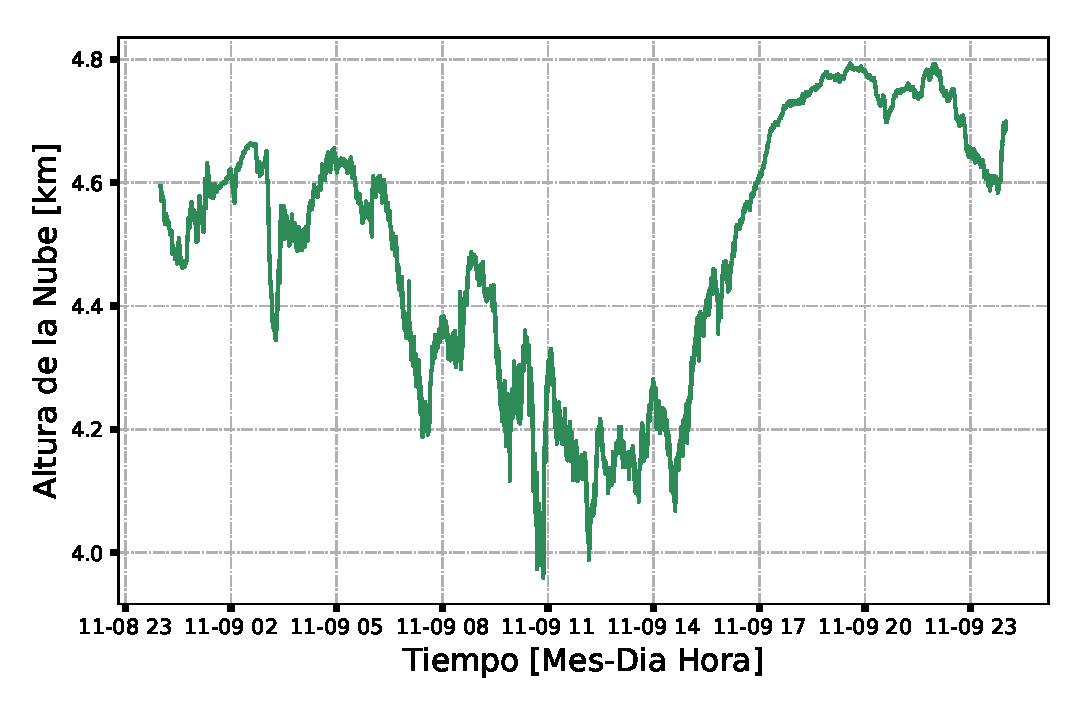
\includegraphics[width=0.8\textwidth]{Figures/Altura_nube.eps}
\caption{Primeras mediciones de altura de la base de la nube, para el día 9 de Noviembre del 2019, el sensor esta ubicado en el observatorio del grupo Halley de la Universidad Industrial de Santander.}
\label{temp}
\end{center}
\end{figure}
En base a las mediciones de temperatura y humedad se presentan en la Fig. \ref{temp}, las primeras valoraciones de altura de la base de la nube para un día lluvioso. Los datos se tomaron el día 9 de Noviembre del 2019, el sensor esta ubicado en el observatorio del grupo Halley de la Universidad Industrial de Santander. \\

\begin{figure}[H]
\begin{center}
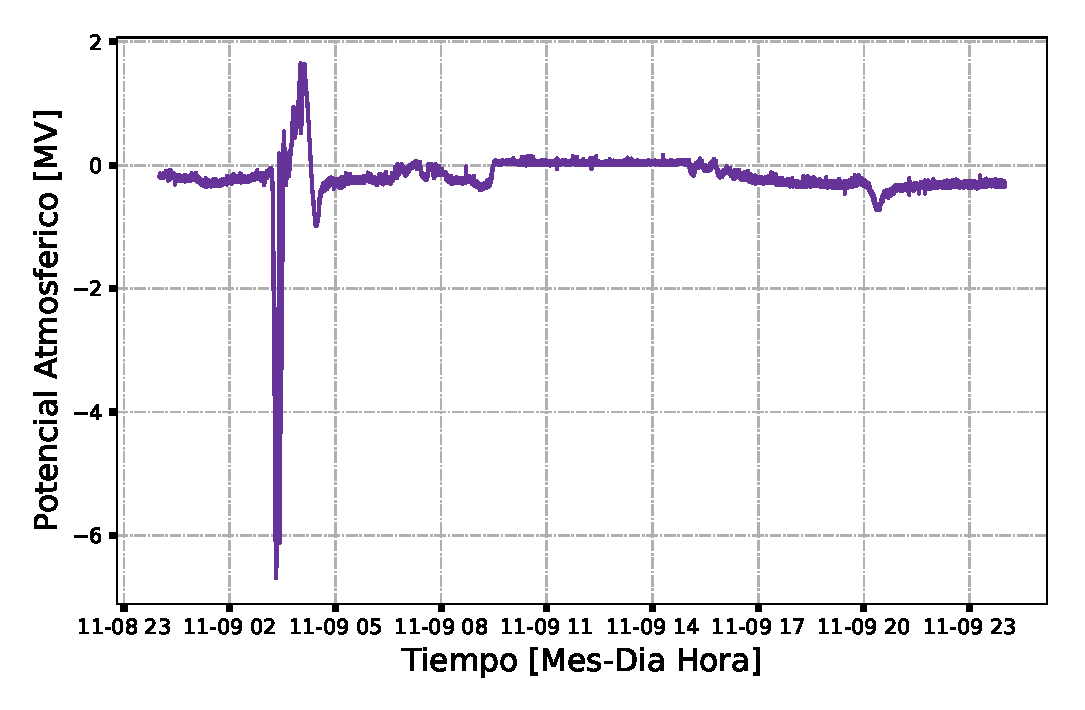
\includegraphics[width=0.8\textwidth]{Figures/potencial.eps}
\caption{Primeras estimaciones del potencial atmosférico, para el día 9 de Noviembre del 2019, el sensor se ubicó en el observatorio del grupo Halley de la Universidad Industrial de Santander.}
\label{pot}
\end{center}
\end{figure}
Sus primeras estimaciones se hicieron en base a la Eq. \ref{potencial}, siendo $E$ el campo eléctrico medido con el sensor de campo lento, y $d$ la altura de la base de la nube. En la Fig. \ref{pot} se presentan la estimación del potencial eléctrico para el día 9 de Noviembre del 2019. Donde se observa la variación que 
  